% ch02_banach.tex — Principe de Contraction de Banach
\chapter{Principe de Contraction de Banach et G\'en\'eralisations}\label{ch:banach}

En 1922, Stefan Banach, un math\'ematicien polonais largement autodidacte,
publie dans sa th\`ese de doctorat un th\'eor\`eme d'une simplicit\'e
\'eblouissante~: si une application \og rapproche\fg{} les points les uns
des autres et si l'espace est complet, alors il existe un unique point fixe,
et on peut le calculer par it\'eration. Ce r\'esultat est devenu l'un des
outils les plus utilis\'es de toute l'analyse~: il d\'emontre l'existence et
l'unicit\'e des solutions d'\'equations diff\'erentielles (Picard-Lindel\"of),
justifie la m\'ethode de Newton, et fonde la r\'esolution de nombreuses
\'equations int\'egrales et fonctionnelles.

% ------------------------------------------------------------
\section{Le th\'eor\`eme fondamental}
% ------------------------------------------------------------

Le principe de contraction de Banach est sans doute le th\'eor\`eme de point fixe
le plus utilis\'e en math\'ematiques. Sa puissance r\'eside dans la conjonction de
trois propri\'et\'es~: existence, unicit\'e et m\'ethode constructive de calcul.

\begin{theoreme}[Principe de Contraction de Banach, 1922]\label{thm:banach}
Soit $(X, d)$ un espace m\'etrique complet et $T : X \to X$ une contraction,
c'est-\`a-dire qu'il existe $k \in [0, 1)$ tel que
\[
    d(T(x), T(y)) \leq k \, d(x, y) \quad \forall x, y \in X.
\]
Alors~:
\begin{enumerate}
    \item $T$ poss\`ede un unique point fixe $x^* \in X$;
    \item Pour tout $x_0 \in X$, la suite d'it\'er\'ees $(T^n(x_0))_{n \geq 0}$
          converge vers $x^*$;
    \item On a les estimations d'erreur~:
    \begin{align}
        d(T^n(x_0), x^*) &\leq \frac{k^n}{1 - k} \, d(x_0, T(x_0))
        \quad \text{(a priori)}, \label{eq:apriori} \\
        d(T^n(x_0), x^*) &\leq \frac{k}{1 - k} \, d(T^{n-1}(x_0), T^n(x_0))
        \quad \text{(a posteriori)}. \label{eq:aposteriori}
    \end{align}
\end{enumerate}
\end{theoreme}

\begin{proof}
\textbf{Existence et convergence.}
Fixons $x_0 \in X$ et posons $x_n = T^n(x_0)$ pour $n \geq 0$. Pour $n \geq 1$,
\[
    d(x_{n+1}, x_n) = d(T(x_n), T(x_{n-1})) \leq k \, d(x_n, x_{n-1})
    \leq \cdots \leq k^n \, d(x_1, x_0).
\]
Pour $m > n$, par l'in\'egalit\'e triangulaire~:
\[
    d(x_m, x_n) \leq \sum_{i=n}^{m-1} d(x_{i+1}, x_i)
    \leq \sum_{i=n}^{m-1} k^i \, d(x_1, x_0)
    \leq \frac{k^n}{1 - k} \, d(x_1, x_0).
\]
Puisque $k < 1$, le membre de droite tend vers $0$ quand $n \to \infty$, donc
$(x_n)$ est une suite de Cauchy. Par compl\'etude de $(X, d)$, elle converge vers
un point $x^* \in X$.

\textbf{Point fixe.}
Par continuit\'e de $T$ (toute contraction est lipschitzienne, donc continue)~:
\[
    T(x^*) = T\left(\lim_{n \to \infty} x_n\right) = \lim_{n \to \infty} T(x_n)
    = \lim_{n \to \infty} x_{n+1} = x^*.
\]

\textbf{Unicit\'e.}
Si $y^*$ est un autre point fixe, alors
\[
    d(x^*, y^*) = d(T(x^*), T(y^*)) \leq k \, d(x^*, y^*).
\]
Puisque $k < 1$, ceci implique $d(x^*, y^*) = 0$, donc $x^* = y^*$.

\textbf{Estimation a priori.}
En faisant $m \to \infty$ dans $d(x_m, x_n) \leq \frac{k^n}{1-k} d(x_1, x_0)$,
on obtient \eqref{eq:apriori}.

\textbf{Estimation a posteriori.}
Pour $m > n$~:
\[
    d(x_m, x_n) \leq \sum_{i=0}^{m-n-1} k^i \, d(x_{n+1}, x_n)
    \leq \frac{1}{1-k} \, d(x_{n+1}, x_n).
\]
En passant \`a la limite $m \to \infty$ et en rempla\c{c}ant $d(x_{n+1}, x_n)$
par $d(T(x_n), T(x_{n-1})) \leq k \, d(x_n, x_{n-1})$, on obtient
\eqref{eq:aposteriori}.
\end{proof}

% Diagramme de convergence en escalier des it\'er\'ees de Banach
\begin{center}
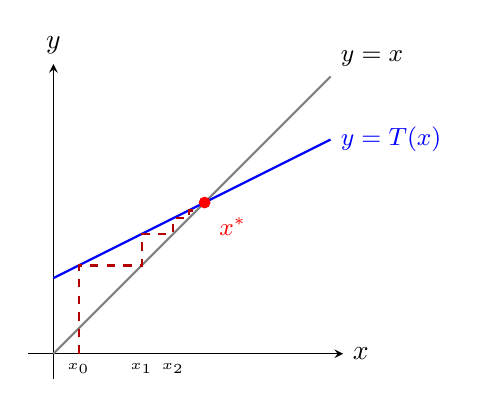
\begin{tikzpicture}[>=stealth, scale=3.2]
  % Axes
  \draw[->] (-0.1,0) -- (1.15,0) node[right] {$x$};
  \draw[->] (0,-0.1) -- (0,1.15) node[above] {$y$};
  % Droite y = x
  \draw[thick, gray] (0,0) -- (1.1,1.1) node[above right, black] {\small $y = x$};
  % Fonction T (contraction) : T(x) = 0.3 + 0.5x
  \draw[thick, blue, domain=0:1.1, samples=50] plot (\x, {0.3 + 0.5*\x})
    node[right] {\small $y = T(x)$};
  % Point fixe x* = 0.6
  \filldraw[red] (0.6,0.6) circle (0.6pt);
  \node[red, below right] at (0.62,0.58) {\small $x^*$};
  % It\'er\'ees en escalier depuis x_0 = 0.1
  % x_0 = 0.1, T(x_0) = 0.35, T^2 = 0.475, T^3 = 0.5375, T^4 = 0.56875
  \draw[thick, dashed, red!70!black]
    (0.1,0) -- (0.1,0.35) -- (0.35,0.35) -- (0.35,0.475)
    -- (0.475,0.475) -- (0.475,0.5375) -- (0.5375,0.5375)
    -- (0.5375,0.56875) -- (0.56875,0.56875) -- (0.56875,0.584);
  % \'Etiquettes
  \node[below] at (0.1,0) {\tiny $x_0$};
  \node[below] at (0.35,0) {\tiny $x_1$};
  \node[below] at (0.475,0) {\tiny $x_2$};
\end{tikzpicture}
\end{center}

\begin{formules}[title=\textbf{Principe de Contraction de Banach}]
Soit $(X, d)$ complet, $T : X \to X$ avec $d(Tx, Ty) \leq k \, d(x,y)$, $k < 1$. Alors~:
\[
    \exists!\, x^* \in X : T(x^*) = x^*, \qquad
    d(T^n x_0, x^*) \leq \frac{k^n}{1-k}\, d(x_0, Tx_0).
\]
\end{formules}

\section{N\'ecessit\'e des hypoth\`eses}

\begin{exemple}[N\'ecessit\'e de la compl\'etude]
Consid\'erons $X = (0, 1]$ muni de la distance usuelle et $T(x) = x/2$.
Alors $T$ est une contraction de constante $1/2$, mais $T$ n'a pas de point
fixe dans $X$ (le point fixe $0$ n'appartient pas \`a $X$). L'espace $(0,1]$
n'est pas complet.
\end{exemple}

\begin{exemple}[N\'ecessit\'e de $k < 1$]
Soit $X = [1, +\infty)$ muni de la distance usuelle et $T(x) = x + 1/x$.
Alors pour $x \neq y$~:
\[
    \abs{T(x) - T(y)} = \abs{x - y} \cdot \abs{1 - \frac{1}{xy}} < \abs{x - y}
\]
donc $T$ est contractante au sens faible ($d(Tx, Ty) < d(x,y)$ pour $x \neq y$),
mais il n'existe pas de $k < 1$ uniforme. L'application $T$ n'a pas de point
fixe dans $[1, +\infty)$.
\end{exemple}

\begin{attention}[title=\textbf{Contraction stricte vs.\ contraction faible}]
La condition $d(Tx, Ty) < d(x,y)$ pour $x \neq y$ (contraction faible) ne
suffit \textbf{pas} pour garantir l'existence d'un point fixe, m\^eme dans un
espace complet. Il faut la condition uniforme $d(Tx, Ty) \leq k \, d(x,y)$
avec $k < 1$ ind\'ependant de $x$ et $y$.
\end{attention}

\section{Vitesse de convergence}

\begin{proposition}[Convergence g\'eom\'etrique]
Sous les hypoth\`eses du Th\'eor\`eme~\ref{thm:banach}, la convergence de $(x_n)$
vers $x^*$ est au moins g\'eom\'etrique de raison $k$~:
\[
    d(x_n, x^*) \leq k \, d(x_{n-1}, x^*) \quad \forall n \geq 1.
\]
\end{proposition}

\begin{proof}
$d(x_n, x^*) = d(T(x_{n-1}), T(x^*)) \leq k \, d(x_{n-1}, x^*)$.
\end{proof}

\begin{remarque}
En pratique, l'estimation a posteriori \eqref{eq:aposteriori} est plus utile
car elle ne n\'ecessite pas de conna\^itre $d(x_0, Tx_0)$ mais seulement la
derni\`ere variation $d(x_{n-1}, x_n)$, qui est calcul\'ee au cours de l'it\'eration.
\end{remarque}

\section{Applications classiques}

\subsection{Th\'eor\`eme de Picard--Lindel\"of}

\begin{theoreme}[Picard--Lindel\"of]
Soient $t_0 \in \R$, $y_0 \in \R^n$, et $f : [t_0 - a, t_0 + a] \times
\overline{B}(y_0, b) \to \R^n$ continue et lipschitzienne en $y$ de constante
$L$. Posons $M = \sup \norm{f}$ et $\delta = \min(a, b/M)$. Si $L\delta < 1$,
alors le probl\`eme de Cauchy
\[
    y'(t) = f(t, y(t)), \quad y(t_0) = y_0
\]
poss\`ede une unique solution sur $[t_0 - \delta, t_0 + \delta]$.
\end{theoreme}

\begin{proof}
Soit $X = C([t_0 - \delta, t_0 + \delta], \overline{B}(y_0, b))$ muni de la
norme $\norm{\cdot}_\infty$. D\'efinissons l'op\'erateur de Picard~:
\[
    (Ty)(t) = y_0 + \int_{t_0}^t f(s, y(s)) \, ds.
\]
V\'erifions que $T$ envoie $X$ dans $X$~: pour $y \in X$,
\[
    \norm{(Ty)(t) - y_0} \leq \int_{t_0}^t \norm{f(s, y(s))} \, ds \leq M\delta \leq b.
\]
V\'erifions que $T$ est une contraction~: pour $y, z \in X$,
\[
    \norm{(Ty)(t) - (Tz)(t)} \leq \int_{t_0}^t L \, \norm{y(s) - z(s)} \, ds
    \leq L\delta \, \norm{y - z}_\infty.
\]
Puisque $L\delta < 1$, le principe de Banach s'applique et fournit l'existence
et l'unicit\'e de la solution.
\end{proof}

\subsection{\'Equations int\'egrales de Fredholm}

\begin{theoreme}[\'Equation de Fredholm]
Soit $K \in C([a,b]^2)$ et $f \in C([a,b])$. Si
$\abs{\lambda} \cdot \sup_{t} \int_a^b \abs{K(t,s)} \, ds < 1$,
alors l'\'equation
\[
    u(t) = f(t) + \lambda \int_a^b K(t,s) \, u(s) \, ds
\]
admet une unique solution dans $C([a,b])$.
\end{theoreme}

\begin{proof}
L'op\'erateur $(Tu)(t) = f(t) + \lambda \int_a^b K(t,s) u(s) \, ds$ est une
contraction sur $(C([a,b]), \norm{\cdot}_\infty)$ de constante
$k = \abs{\lambda} \sup_t \int_a^b \abs{K(t,s)} \, ds < 1$.
\end{proof}

\subsection{Th\'eor\`eme d'inversion locale}

\begin{theoreme}[Inversion locale via Banach]
Soit $E$ un espace de Banach et $F : E \to E$ de classe $C^1$ avec
$DF(x_0)$ inversible. Alors $F$ est un diff\'eomorphisme local au voisinage de $x_0$.
\end{theoreme}

\begin{proof}[Id\'ee de la preuve]
Sans perte de g\'en\'eralit\'e, $x_0 = 0$ et $DF(0) = \mathrm{Id}$, donc
$F(x) = x - \varphi(x)$ avec $D\varphi(0) = 0$. Pour $y$ proche de $0$,
l'\'equation $F(x) = y$ s'\'ecrit $x = y + \varphi(x) = T_y(x)$.
Par continuit\'e de $D\varphi$, $T_y$ est une contraction sur une boule
suffisamment petite autour de $0$.
\end{proof}

\section{G\'en\'eralisations directes}

\subsection{Contractions sur un ferm\'e}

\begin{proposition}[Contraction sur un ferm\'e]
Soit $(X, d)$ un espace m\'etrique complet et $F \subset X$ un ferm\'e non vide.
Si $T : F \to F$ est une contraction, alors $T$ admet un unique point fixe
dans $F$.
\end{proposition}

\begin{proof}
Un ferm\'e d'un espace complet est complet, et on applique le
Th\'eor\`eme~\ref{thm:banach}.
\end{proof}

\subsection{It\'er\'ee contractante}

\begin{theoreme}[It\'er\'ee contractante]
Soit $(X, d)$ un espace m\'etrique complet et $T : X \to X$ continue.
Si $T^N$ est une contraction pour un certain $N \geq 1$, alors $T$ poss\`ede
un unique point fixe.
\end{theoreme}

\begin{proof}
Par le th\'eor\`eme de Banach appliqu\'e \`a $T^N$, il existe un unique $x^*$ tel
que $T^N(x^*) = x^*$. Alors $T^N(T(x^*)) = T(T^N(x^*)) = T(x^*)$, donc
$T(x^*)$ est aussi un point fixe de $T^N$. Par unicit\'e, $T(x^*) = x^*$.

R\'eciproquement, tout point fixe de $T$ est un point fixe de $T^N$, donc $T$
a un unique point fixe.
\end{proof}

\begin{exemple}
L'application $T : C([0,1]) \to C([0,1])$ d\'efinie par
$(Tf)(x) = \int_0^x f(t) \, dt$ n'est pas contractante, mais $T^N$ est
contractante pour $N$ assez grand car $\norm{T^N f}_\infty \leq
\frac{\norm{f}_\infty}{N!}$.
\end{exemple}

\subsection{Principe de Banach avec param\`etre}

\begin{theoreme}[D\'ependance continue par rapport \`a un param\`etre]
Soit $(X, d)$ un espace m\'etrique complet, $\Lambda$ un espace topologique, et
$T : X \times \Lambda \to X$ telle que~:
\begin{enumerate}
    \item Pour tout $\lambda \in \Lambda$, $T(\cdot, \lambda)$ est une contraction
          de constante $k < 1$ (uniforme en $\lambda$);
    \item Pour tout $x \in X$, $T(x, \cdot) : \Lambda \to X$ est continue.
\end{enumerate}
Alors l'application $\lambda \mapsto x^*(\lambda)$, o\`u $x^*(\lambda)$ est
l'unique point fixe de $T(\cdot, \lambda)$, est continue.
\end{theoreme}

\begin{proof}
Soient $\lambda_0 \in \Lambda$ et $\varepsilon > 0$. On a~:
\begin{align*}
    d(x^*(\lambda), x^*(\lambda_0))
    &= d(T(x^*(\lambda), \lambda), T(x^*(\lambda_0), \lambda_0)) \\
    &\leq d(T(x^*(\lambda), \lambda), T(x^*(\lambda_0), \lambda))
         + d(T(x^*(\lambda_0), \lambda), T(x^*(\lambda_0), \lambda_0)) \\
    &\leq k \, d(x^*(\lambda), x^*(\lambda_0))
         + d(T(x^*(\lambda_0), \lambda), T(x^*(\lambda_0), \lambda_0)).
\end{align*}
Donc $(1-k) \, d(x^*(\lambda), x^*(\lambda_0)) \leq
d(T(x^*(\lambda_0), \lambda), T(x^*(\lambda_0), \lambda_0))$. Le membre de
droite tend vers $0$ quand $\lambda \to \lambda_0$ par l'hypoth\`ese (2).
\end{proof}

\section{Th\'eor\`eme de Banach--Caccioppoli g\'en\'eralis\'e}

\begin{theoreme}[Contraction sur boule]
Soit $(X, d)$ un espace m\'etrique complet, $x_0 \in X$, $r > 0$, et
$T : \overline{B}(x_0, r) \to X$ une contraction de constante $k < 1$. Si
\[
    d(x_0, T(x_0)) < (1 - k) r,
\]
alors $T$ admet un unique point fixe dans $\overline{B}(x_0, r)$.
\end{theoreme}

\begin{proof}
Il suffit de montrer que $T(\overline{B}(x_0, r)) \subset \overline{B}(x_0, r)$.
Pour $x \in \overline{B}(x_0, r)$~:
\[
    d(T(x), x_0) \leq d(T(x), T(x_0)) + d(T(x_0), x_0)
    \leq k \, d(x, x_0) + d(T(x_0), x_0) \leq kr + (1-k)r = r.
\]
On applique alors le th\'eor\`eme de Banach \`a $T : \overline{B}(x_0, r) \to
\overline{B}(x_0, r)$.
\end{proof}

\section{Applications non expansives}

\begin{definition}[Application non expansive]
Une application $T : X \to X$ est \emph{non expansive} si
$d(T(x), T(y)) \leq d(x, y)$ pour tous $x, y \in X$.
\end{definition}

\begin{remarque}
Une application non expansive n'a pas n\'ecessairement de point fixe, m\^eme dans
un espace complet. Par exemple, la translation $T(x) = x + 1$ sur $\R$ est
non expansive sans point fixe.
\end{remarque}

\begin{theoreme}[Browder--G\"ohde--Kirk, 1965]
Soit $C$ un sous-ensemble convexe, born\'e et ferm\'e d'un espace de Hilbert $H$.
Si $T : C \to C$ est non expansive, alors $T$ poss\`ede un point fixe.
\end{theoreme}

\begin{proof}[Id\'ee de la preuve]
Pour $\lambda \in (0,1)$, fixons $a \in C$ et d\'efinissons
$T_\lambda(x) = \lambda a + (1-\lambda) T(x)$. Alors $T_\lambda$ est une
contraction de constante $1 - \lambda$ et envoie $C$ dans $C$ par convexit\'e.
Soit $x_\lambda$ son unique point fixe~:
\[
    x_\lambda = \lambda a + (1-\lambda) T(x_\lambda).
\]
Quand $\lambda \to 0^+$, on montre (en utilisant la structure hilbertienne)
que $(x_\lambda)$ converge faiblement vers un point fixe de $T$.
\end{proof}

\section{Contractions g\'en\'eralis\'ees de Boyd--Wong}

\begin{theoreme}[Boyd--Wong, 1969]
Soit $(X, d)$ un espace m\'etrique complet et $T : X \to X$ v\'erifiant
\[
    d(T(x), T(y)) \leq \psi(d(x, y)) \quad \forall x, y \in X,
\]
o\`u $\psi : [0, \infty) \to [0, \infty)$ est semi-continue sup\'erieurement
\`a droite et satisfait $\psi(t) < t$ pour tout $t > 0$.
Alors $T$ admet un unique point fixe.
\end{theoreme}

\begin{proof}
Fixons $x_0 \in X$ et posons $x_n = T^n(x_0)$. La suite $(d_n)$ d\'efinie par
$d_n = d(x_n, x_{n+1})$ est d\'ecroissante car $d_{n+1} \leq \psi(d_n) < d_n$
si $d_n > 0$. Elle converge donc vers une limite $\ell \geq 0$.

Si $\ell > 0$, par semi-continuit\'e sup\'erieure \`a droite de $\psi$~:
$\ell \leq \limsup_{n} \psi(d_n) \leq \psi(\ell) < \ell$, contradiction. Donc
$\ell = 0$.

Montrons que $(x_n)$ est de Cauchy. Raisonnons par l'absurde~: il existerait
$\varepsilon > 0$ et des sous-suites $m(k) > n(k) \to \infty$ avec
$d(x_{m(k)}, x_{n(k)}) \geq \varepsilon$. On peut choisir $m(k)$ minimal,
donc $d(x_{m(k)-1}, x_{n(k)}) < \varepsilon$. Alors
\begin{align*}
    \varepsilon &\leq d(x_{m(k)}, x_{n(k)})
    \leq d(x_{m(k)}, x_{m(k)-1}) + d(x_{m(k)-1}, x_{n(k)})
    < d_{m(k)-1} + \varepsilon.
\end{align*}
Donc $d(x_{m(k)}, x_{n(k)}) \to \varepsilon$. Par le caract\`ere contractant~:
\[
    d(x_{m(k)+1}, x_{n(k)+1}) \leq \psi(d(x_{m(k)}, x_{n(k)})).
\]
En passant \`a la limite~: $\varepsilon \leq \psi(\varepsilon) < \varepsilon$,
contradiction. Donc $(x_n)$ est de Cauchy.

Par compl\'etude, $x_n \to x^*$, et par continuit\'e de $T$ (cons\'equence de
l'hypoth\`ese), $T(x^*) = x^*$. L'unicit\'e se d\'emontre comme pour Banach.
\end{proof}

\section{Contractions de Meir--Keeler}

\begin{theoreme}[Meir--Keeler, 1969]
Soit $(X, d)$ un espace m\'etrique complet et $T : X \to X$ v\'erifiant~:
pour tout $\varepsilon > 0$, il existe $\delta > 0$ tel que
\[
    \varepsilon \leq d(x, y) < \varepsilon + \delta \implies d(T(x), T(y)) < \varepsilon.
\]
Alors $T$ admet un unique point fixe.
\end{theoreme}

\begin{remarque}
La condition de Meir--Keeler implique $d(Tx, Ty) < d(x,y)$ pour $x \neq y$
(prendre $\varepsilon = d(x,y)$), mais elle est strictement plus forte qu'une
simple contraction faible. Toute contraction de Banach (constante $k < 1$)
v\'erifie la condition de Meir--Keeler avec $\delta = \varepsilon(1-k)/k$.
\end{remarque}

\section{Th\'eor\`eme de point fixe de Matkowski}

\begin{theoreme}[Matkowski, 1975]
Soit $(X, d)$ un espace m\'etrique complet et $T : X \to X$ v\'erifiant
\[
    d(T(x), T(y)) \leq \psi(d(x, y)) \quad \forall x, y \in X,
\]
o\`u $\psi : [0, \infty) \to [0, \infty)$ est croissante et satisfait
$\lim_{n \to \infty} \psi^n(t) = 0$ pour tout $t > 0$.
Alors $T$ admet un unique point fixe.
\end{theoreme}

\begin{remarque}
Notons que si $\psi$ est croissante et $\psi^n(t) \to 0$, alors $\psi(t) < t$
pour tout $t > 0$. En effet, si $\psi(t_0) \geq t_0$ pour un $t_0 > 0$,
alors par croissance $\psi^n(t_0) \geq t_0$ pour tout $n$, contredisant
$\psi^n(t_0) \to 0$.
\end{remarque}

\section{Exercices}

\begin{exercice}
Soit $T : \R \to \R$ d\'efinie par $T(x) = \frac{1}{2}(x + a/x)$ pour $x > 0$,
o\`u $a > 0$. Montrer que pour tout $x_0 > 0$, la suite $(T^n(x_0))$ converge
vers $\sqrt{a}$. S'agit-il d'une contraction de Banach~?
\end{exercice}

\begin{exercice}
Montrer que l'application $T : C([0,1]) \to C([0,1])$ d\'efinie par
$(Tf)(x) = \int_0^x f(t) \, dt$ n'est pas une contraction, mais que $T^n$ est
une contraction pour $n \geq 2$. En d\'eduire que $T$ a un unique point fixe
(la fonction nulle).
\end{exercice}

\begin{exercice}
Soit $(X, d)$ un espace m\'etrique complet et $T : X \to X$ telle que
$d(T(x), T(y)) \leq \alpha \, d(x, T(x)) + \beta \, d(y, T(y))$ avec
$\alpha + \beta < 1$. Montrer que $T$ admet un unique point fixe.
\textit{C'est la condition de Kannan, \'etudi\'ee au Chapitre~3.}
\end{exercice}

\begin{exercice}
Soit $A$ une matrice $n \times n$ avec $\norm{A} < 1$ (norme d'op\'erateur).
Montrer que $(I - A)$ est inversible et que $(I - A)^{-1} = \sum_{k=0}^\infty A^k$
(s\'erie de Neumann). D\'emontrer ce r\'esultat en utilisant le principe de Banach.
\end{exercice}

\begin{exercice}[Th\'eor\`eme de Nadler]
Soit $(X, d)$ un espace m\'etrique complet et $T : X \to \mathcal{K}(X)$ une
application multivoque \`a valeurs compactes non vides, contractante pour la
m\'etrique de Hausdorff~:
\[
    H(T(x), T(y)) \leq k \, d(x, y), \quad k < 1.
\]
Montrer que $T$ poss\`ede un point fixe, c'est-\`a-dire un $x^*$ tel que
$x^* \in T(x^*)$.
\end{exercice}

\begin{exercice}
Soit $f : \R^n \to \R^n$ de classe $C^1$ telle que $\norm{Df(x)} \leq k < 1$
pour tout $x$ (norme d'op\'erateur). Montrer que $f$ est une contraction et en
d\'eduire que l'\'equation $x = f(x)$ a une unique solution.
\end{exercice}

\begin{exercice}
\'Etudier la convergence de la m\'ethode de Newton comme cas particulier du
principe de contraction. Pr\'ecis\'ement, soit $g : \R \to \R$ de classe $C^2$
avec $g(x^*) = 0$ et $g'(x^*) \neq 0$. Montrer que l'it\'eration
$x_{n+1} = x_n - g(x_n)/g'(x_n)$ converge vers $x^*$ pour $x_0$ suffisamment
proche de $x^*$, et que la convergence est quadratique.
\end{exercice}
